\section { Computer Vision }
	\subsection { The pinhole camera model }
		Cameras project 3-dimensional scenes onto a 2-dimensional plane - the image plane.
		The overall projection of a single point in space (given in a world copordinate system) to the image plane can be divided into two independent successive operations \cite[S.~50]{Szeliski2010}:
		
		\subsubsection{Extrinsic parameters}
		A camera's extrinsic parameters describe its position and pose relative to the world coordinate system. For a simple pinhole camera those parameters are given with 
		
		\begin{equation}
		\matr{C} = \begin{bmatrix}
					\matr{R}_{3\times 3} & T_{3\times 1}\\
					0_{1\times 3} & 1
					\end{bmatrix}_{4\times 4} = -\matr{R}^{-1}T = -\matr{R}^TT \, . 
		\end{equation}
		$\matr{R}_{3\times 3}$ is a rotation matrix that represents the camera's rotation relative to the world coordinate system and T is the position of the world coordinate system, given in the new, camera-centered coordinate system. 

		\subsection{Intrinsic parameters}
		A camera intrinsic parameters reflect its internal structure and depend on focal length $f_{2\times 1}$, size of the image sensor and the principal point $c_{2\times1}$ which is defined as the intersection of the camera's optical axis with the image plane, denoted in pixel coordinates. This point ideally corresponds with the image sensor's center but might be slightly offset because of small misalignments within the camera.
		
		All in all this results in the camera's intrinsic matrix
		\begin{equation}
		\matr{K} =	\begin{bmatrix}
			f_x & s & c_x & 0 \\
			0 & f_y & c_y & 0 \\
			0 & 0 & 1 & 0
			\end{bmatrix}.
		\end{equation}
		The factor $s$ encodes any possible skew that might be introduced through misalignments between the camera's sensor and its optical axis and can typically be set to $0$ without affecting the approximation of the camera model too much.
		
		\subsection{Combined model}
		Combined, the intrinsic and extrinsic matrices lead to a camera matrix \cite{Szeliski2010}:
		
		\begin{equation}
		\matr{P} = \begin{bmatrix}\matr{K} & 0\\\matr{0}^T & 1\end{bmatrix}
		\begin{bmatrix}\matr{R} & T\\\matr{0}^T & 1\end{bmatrix}
		\end{equation}
		
		which maps a point $p_w = \left(x_w, y_w, z_w, 1\right)$ given in world coordinates to screen coordinates and disparity $d$, $p_s = \left(x_s, y_s, 1, d\right)$.
		
		
	\subsection { Segmentierung }
		

	
\section { Machine Learning }

		
	In recent years, there has been steady progress in the performance of computing hardware and thus in the area of machine learning.
In this section the machine-learning techniques used in the work are briefly shown and explained.

	\subsection { Neuronale Netze }
	Artificial neural networks 	are modeled on the biological function of human nerve tracts.

		\subsubsection { Das Perzeptron }
		\begin{figure}
								\tikzset{%
				every neuron/.style={
					circle,
					draw,
					minimum size=1cm
				},
				neuron missing/.style={
					draw=none, 
					scale=1,
					text height=0.333cm,
					execute at begin node=\color{black}$\vdots$
				},
			}
			
			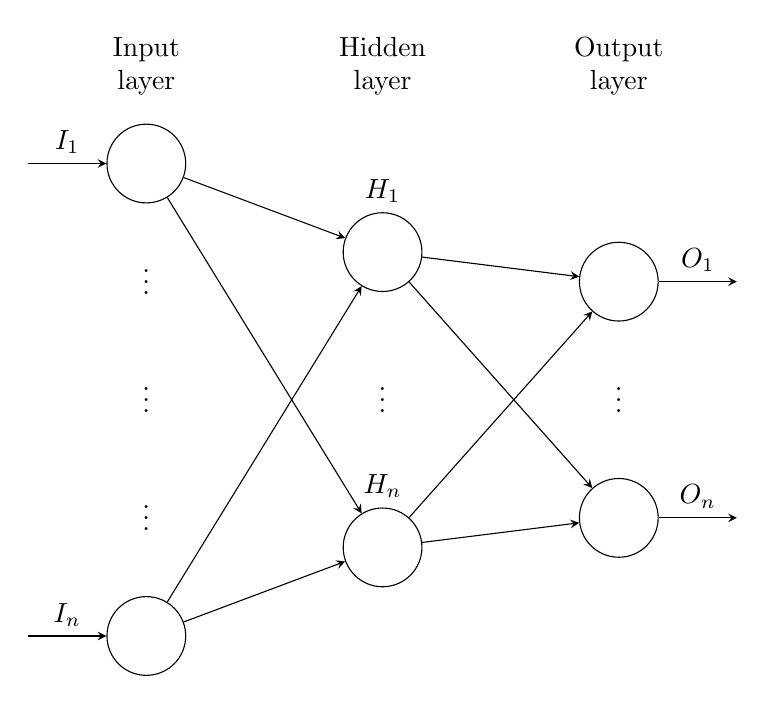
\begin{tikzpicture}[x=1.5cm, y=1.5cm, >=stealth]
			
			\foreach \m/\l [count=\y] in {1,missing, missing, missing, 5}
			\node [every neuron/.try, neuron \m/.try] (input-\y) at (0,2.5-\y) {};
			
			\foreach \m [count=\y] in {1,missing,2}
			\node [every neuron/.try, neuron \m/.try ] (hidden-\m) at (2,2-\y*1.25) {};
			
			\foreach \m [count=\y] in {1,missing,2}
			\node [every neuron/.try, neuron \m/.try ] (output-\m) at (4,1.5-\y) {};
			
			
			\draw [<-] (input-1) -- ++(-1,0)
			node [above, midway] {$I_1$};
			
			\draw [<-] (input-5) -- ++(-1,0)
			node [above, midway] {$I_n$};
			
			\foreach \l [count=\i] in {1,n}
			\node [above] at (hidden-\i.north) {$H_\l$};
			
			\foreach \l [count=\i] in {1,n}
			\draw [->] (output-\i) -- ++(1,0)
			node [above, midway] {$O_\l$};
			
			\foreach \i in {1,5}
			\foreach \j in {1,...,2}
			\draw [->] (input-\i) -- (hidden-\j);
			
			\foreach \i in {1,...,2}
			\foreach \j in {1,...,2}
			\draw [->] (hidden-\i) -- (output-\j);
			
			\foreach \l [count=\x from 0] in {Input, Hidden , Output}
			\node [align=center, above] at (\x*2,2) {\l \\ layer};
			
			\end{tikzpicture}
					\centering
			\caption{Structure of a simple multi layer perceptron with one hidden layer.}
		\end{figure}
		The perceptron is the simplest case of a neural network. It consists of at least two layers with any number of arithmetic units called neurons with the first and last layer playing a special role since they are connected to the "`outside"' and transfer data into and out of the network. The layers in between are called "`hidden layers"'.
		
		All neurons of one layer are fully connected to every neuron of the following layer via a weighted connection:
		
		Each arithmetic unit in layer $j$ takes the data $o_{j-1} = o_i$ from the preceding neurons and calculates a preliminary output value $net_j$ by multiplying each input with the corresponding weights $w_{ij}$:
		
		 \ref{eq:perceptron_simple}. 
		
		\begin{equation}
			\label{eq:perceptron_simple}
			\text{net}_j = \sum_{i=1}^{n} w_{ij} \cdot o_i + b \, . 
		\end{equation}
		
		The weights $w_{xy}$ and bias values $b_x$ are optimized in the training process to approximate the training data as close as possible and will not change after the training.
		
		
		The inputs for the next layer are then calculated by filtering the preliminary results through a non-linear activation function,
		
		\begin{equation}
		\label{eq:perceptron_act}
		o_j = \varphi\left(\text{net}_j\right) \, . 
		\end{equation}
		

		
		 
		\subsubsection { Aktivierungsfunktionen }
		Since the basic arithmetic operations in a neural network are linear in nature, an additional nonlinearity must be introduced in order to learn nonlinear correlations. 
For this purpose different activation functions $\varphi$ are used, some of which are explained in the following.\\

		
		\textbf{Schwellenwertfunktion}
		Die Schwellenwertfunktion ist die ursprüngliche Aktivierungsfunktion für das Perzeptron nach \cite{McCulloch1943} und besitzt lediglich $0$ und $1$ als mögliche Ausgangswerte. Sie ist mit dem Schwellenwert $\epsilon$ definiert zu 
		\begin{equation}
		\label{eq:acti_sw}
		o_j = \left\{
		\begin{array}{ll}
		1\text{, wenn } \text{net}_j > \epsilon \\
		0 \text{ sonst}\\
		\end{array}
		\right.
		\end{equation}
		\textbf{Sigmoid}
			Die Sigmoid-Funktion ist mit einem variablen Steigungsparameter $a$ definiert zu 
			\begin{equation}
			\varphi\left(\text{net}_j\right) = \frac{1}{1+\exp(-a \cdot \text{net}_j)}
			\end{equation}
			Sie wird häufig anstatt der Schwellenwertfunktion genutzt, da sie stetig differenzierbar und somit gut geeignet für häufig genutzte Trainingsverfahren wie Gradient Descend ist.\\
			\begin{figure}[ht]
				\centering
				\begin{tikzpicture}
				\begin{axis}[
				domain=-200:200,
				xmin=-10, xmax=10,
				ymin=-1.5, ymax=1.5,
				samples=401,
				axis y line=center,
				axis x line=middle,
				]
				\addplot+[mark=none] {1/(1 + exp(-x)};
				\end{axis}
				\end{tikzpicture}
				\caption{Die Sigmoid-Funktion begrenzt die Ausgangswerte wie auch die Schwellenwertfunktion auf den Bereich [0, 1].}
				\label{fig:sigmoid_plot}
			\end{figure}


		\textbf{ReLu}
		Die Rectifying linear unit (kurz: ReLu) ist eine weitere Form der Aktivierungsfunktion, die insbesondere in Deep Neural Networks und Convolutional Neural Networks eingesetzt wird. Sie ist definiert zu
		\begin{equation}
			\label{eq:relu_def}
			\varphi(\text{net}_j) = \max(\text{net}_j, 0)
		\end{equation}
		womit negative Werte abgeschnitten werden. Im Vergleich zur Schwellenwert- bzw. Sigmoidfunktion führen große Eingangswerte hier nicht zur Sättigung (und damit kleinem Gradienten), was insbesondere in Gradientenverfahren wie in Abschnitt \ref{sec:gradient-descend} von Vorteil ist. \\
		
		\begin{figure}[ht]
			\centering
		\begin{tikzpicture}
		\begin{axis}[
		domain=-200:200,
		xmin=-10, xmax=10,
		ymin=-10, ymax=10,
		samples=401,
		axis y line=center,
		axis x line=middle,
		]
		\addplot+[mark=none] {max(x, 0)};
		\end{axis}
		\end{tikzpicture}
		\caption{Durch die ReLu-Aktivierungsfunktion werden negative Werte abgeschnitten.}
		\label{fig:relu_plot}
		\end{figure}

	
	\subsection { Spezialfälle Neuronaler Netze}
		\subsubsection { Convolutional Neural Networks (CNN) }
		Convolutional neural networks (\abbrev{CNN}) are a special case of neural networks that are particularly suitable for processing higher-dimensional structures such as images or temporal sequences of data. 

		In a CNN, in addition to the "`dense"' or "`fully connected"' layers described above, additional layers are used that perform convolution operations on the data.

		Instead of a simple multiplication, each input tensor is convoluted with a matrix in each convolution layer.

		In the case of a 2D CNN, the input data is a 2D matrix and each convolution layer also contains several two-dimensional matrices, which are moved over the input matrix to calculate the output data. 

		
		\todo{Bild für Faltung}
		
		
		\subsubsection { Recurrent Neural Networks (RNN) }
		\subsubsection { Long Short Term Memory (LSTM) }
	
	\subsection { Trainingsmethoden }
		
		\subsubsection{Gradient Descend}
		\label{sec:gradient-descend}
		
		\subsubsection{ADAM}
		\todo{Link zum Paper ist in tensorflow source von adam optimizer zu finden}
		
	\subsection{ One Shot Learning - Siamesische Netze }
	Ein Problem der bisher gezeigten Machine Learning-Methoden ist, dass sehr viele Traningsdaten benötigt werden, um die Netze ausreichend zu trainieren. In Anwendungsfällen, in denen die Trainingsdaten erst in der Benutzerinteraktion zur Verfügung stehen, können jedoch häufig nicht ausreichend viele Daten gesammelt werden. 
	
	Ein klassischer Anwendungsfall für One Shot learning ist daher zum Beispiel die Gesichtserkennung in Anwendersoftware. Hier muss es möglich sein, mit wenigen Gesichtern als Vorlage ein Gesicht auf einem neuen Photo zuverlässig wiederzuerkennen. Gleichzeitig sollte es jeder Zeit möglich sein, neue Klassen hinzuzufügen oder alte Klassen zu entfernen. Auch hier ist ein klassisches Netzwerk mit einer festen Anzahl von Ausgangsneuronen - und damit Klassen - ungeeignet.

	\subsubsection{Funktionsprinzip}
		Siamesische Netze sind eine mögliche Lösung für beide genannten Probleme: Sie vergleichen zwei Eingangstensoren und errechnen aus diesen einen Ähnlichkeitsfaktor. Anhand dieses Faktors kann nach Vergleich des unbekannten Eingangs mit allen bekannten Klassen diejenige mit der höchsten Übereinstimmung (oder keine im Fall eines Negativbeispiels) gewählt werden.
		
	\subsubsection{Aufbau des Netzes}
	 Bei einem Siamesischen Netzwerk handelt es sich um ein zweistufiges Netz, bestehend aus zwei Faltungsnetzen mit identischen Gewichten in der ersten Stufe, deren Ergebnis-Vektoren in der zweiten Stufe durch ein zusammenfassendes mehrlagiges Perzeptron in einen einzelnen Ähnlichkeits-Wert umgerechnet werden.
	 Die Faltungsnetze dienen dabei der Dimensionsreduktion - sie reduzieren den Eingangstensor auf einen Festure-Vektor und komprimieren damit die zur Verfügung stehende Information \todo{weiter}
	 
	 
	 
	 \begin{figure}
	 	\centering
	 	 \newcommand*{\h}{\hspace{5pt}}% for indentation
 \newcommand*{\hh}{\h\h}% double indentation
  \begin{tikzpicture}[auto,
    %decision/.style={diamond, draw=black, thick, fill=white,
    %text width=8em, text badly centered,
    %inner sep=1pt, font=\sffamily\small},
    block_center/.style ={rectangle, draw=black, thick, fill=white,
      text width=8em, text centered,
      minimum height=4em},
    block_left/.style ={rectangle, draw=black, thick, fill=white,
      text width=16em, text ragged, minimum height=4em, inner sep=6pt},
    block_noborder/.style ={rectangle, draw=none, thick, fill=none,
      text width=18em, text centered, minimum height=1em},
    block_assign/.style ={rectangle, draw=black, thick, fill=white,
      text width=18em, text ragged, minimum height=3em, inner sep=6pt},
    block_lost/.style ={rectangle, draw=black, thick, fill=white,
      text width=16em, text ragged, minimum height=3em, inner sep=6pt},
      line/.style ={draw, thick, -latex', shorten >=0pt}]
    % outlining the flowchart using the PGF/TikZ matrix funtion
    \matrix [column sep=5mm,row sep=3mm] {
      % enrollment - row 1
      \node [block_center] (referred) {Referred (n=173)};
      & \node [block_left] (excluded1) {Excluded (n=17): \\
        a) Did not wish to participate (n=9) \\
        b) Did not show for interview (n=5) \\
        c) Other reasons (n=3)}; \\
      % enrollment - row 2
      \node [block_center] (assessment) {Assessed for eligibility (n=156)}; 
      & \node [block_left] (excluded2) {Excluded (n=54): \\
        a) Inclusion criteria not met (n=22) \\
        b) Exclusion criteria(s) met (n=13) \\
        c) Not suited for group (n=7) \\
        d) Not suited for CBT (n=2) \\
        e) Sought other treatment (n=3) \\
        f) Other reasons (n=7)}; \\
      % enrollment - row 3
      \node [block_center] (random) {Randomised (n=102)}; 
      & \\
      % follow-up - row 4
      \node [block_noborder] (i) {Intervention group}; 
      & \node [block_noborder] (wlc) {Wait-list control group}; \\
      % follow-up - row 5
      \node [block_assign] (i_T0) {Allocated to intervention (n=51): \\
      \h Received intervention (n=49) \\
      \h Did not receive intervention (n=2, \\
      \hh 1 with primary anxiety disorder, \\
      \hh 1 could not find time to participate)}; 
	  & \node [block_assign] (wlc_T0) {Allocated to wait-list (n=51): \\
      \h Stayed on wait-list (n=48) \\
      \h Did not stay on wait-list (n=3, \\
      \hh 2 changed jobs and lost motivation, \\
      \hh 1 was offered treatment elsewhere)}; \\
      % follow-up - row 6
      \node [block_lost] (i_T3) {Post-intervention measurement: \\
      \h Lost to follow-up (n=5, \\
      \hh 2 dropped out of the intervention, \\
      \hh 3 did not complete measurement)}; 
	  & \node [block_lost] (wlc_T3) {Post-wait-list measurement: \\
      \h Lost to follow-up (n=6, \\
      \hh 3 dropped out of the wait-list, \\
      \hh 3 did not complete measurement)}; \\
      % follow-up - row 7
      % empty first column for intervention group 
      & \node [block_assign] (wlc_T36) {Allocated to intervention (n=48): \\
      \h Received intervention (n=46) \\
      \h Did not receive intervention (n=2, \\
      \hh 1 reported low motivation, \\
      \hh 1 could not find time to participate)}; \\
      % follow-up - row 8
      \node [block_lost] (i_T6) {3-months follow-up measurement: \\
      \h Lost to follow-up (n=9, \\
      \hh did not complete measurement)}; 
      & \node [block_lost] (wlc_T6) {Post-intervention measurement: \\
      \h Lost to follow-up (n=5, \\
      \hh 2 dropped out of the intervention, \\
      \hh 3 did not complete measurement)}; \\
      % follow-up - row 9
      % empty first column for intervention group 
      & \node [block_lost] (wlc_T9) {3-months follow-up measurement \\
      \h Lost to follow-up (n=2, \\
      \hh did not complete measurement)}; \\
      % analysis - row 10
      \node [block_assign] (i_ana) {Analysed (n=51)}; 
      & \node [block_assign] (wlc_ana) {Analysed (n=51)}; \\
    };% end matrix
    % connecting nodes with paths
    \begin{scope}[every path/.style=line]
      % paths for enrollemnt rows
      \path (referred)   -- (excluded1);
      \path (referred)   -- (assessment);
      \path (assessment) -- (excluded2);
      \path (assessment) -- (random);
      \path (random)     -- (i);
      \path (random)     -| (wlc);
      % paths for i-group follow-up rows
      \path (i)          -- (i_T0);
      \path (i_T0)       -- (i_T3);
      \path (i_T3)       -- (i_T6);
      \path (i_T6)       -- (i_ana);
      % paths for wlc-group follow-up rows
      \path (wlc)        -- (wlc_T0);
      \path (wlc_T0)     -- (wlc_T3);
      \path (wlc_T3)     -- (wlc_T36);
      \path (wlc_T36)    -- (wlc_T6);
      \path (wlc_T6)     -- (wlc_T9);
      \path (wlc_T9)     -- (wlc_ana);
    \end{scope}
  \end{tikzpicture}

	 	\caption{Aufbau eines siamesischen Netzwerkes}
	 	\label{fig:siamesenetwork}
	 \end{figure}
	 
	 
	 \subsubsection{Training}
	 Aufgrund des zweistufigen Aufbaus kann auch das Training des Netzes in zwei Stufen erfolgen.
	 
	 \subsubsection{Kostenfunktion: Triplet Loss}
	 Da das Netzwerk \todo{weiter}
	 

	
	Hierfür kann ein Siamesisches Netzwerk (en.: siamese network) genutzt werden. 
	
\section { Anatomie der menschlichen Hand }
	Die Bewegungsfreiheit der einzelnen Handglieder unterliegt anatomischen Beschränkungen, die in der Posenschätzung nützlich sein können, um die Güte der Schätzung zu beurteilen und mit einem passenden Modell entsprechend verfeinern zu können \cite{Melax5222017}.
	
	\begin{figure}
		\centering
		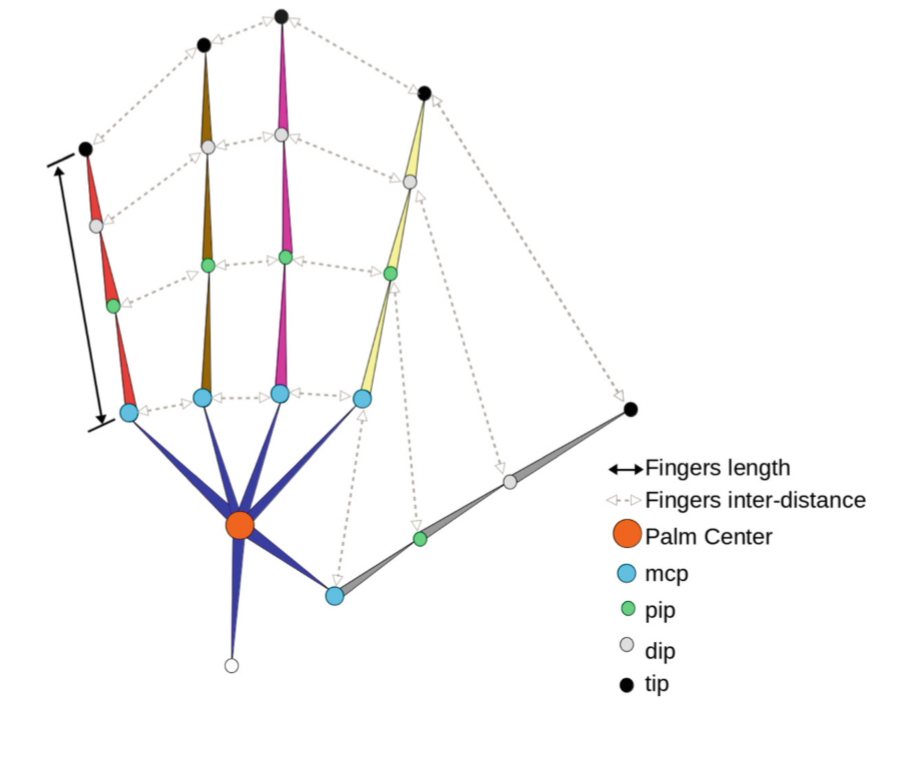
\includegraphics[width=0.7\linewidth]{Ressourcen/malik2018_hand_model}
		\caption[Handmodell nach \cite{Malik2018b}]{In \cite{Malik2018b} wird ein Modell ähnlich dem oben stehenden (Quelle: \cite{Malik2018b}) genutzt, in dem die vollständige Handpose durch 21, bzw. 22 (Gelenk-) Koordinaten bestimmt ist.}
		\label{fig:malik2018handmodel}
	\end{figure}
	
	
	\subsection{title}
	
	
\section{Kameraparameter}
\subsection{Intrinsische Parameter}
Die intrinsischen Paramter einer Kamera sind definiert durch die Brennweite $f$, das Format des Bildsensors und 
\subsection{Extrinsische Parameter}
	